\documentclass[11pt,a4paper]{article}

\usepackage[a4paper,margin=24mm,headheight=14pt]{geometry}
\usepackage[T1]{fontenc}
\usepackage[utf8]{inputenc}
\usepackage{lmodern}
\usepackage{graphicx}
\usepackage{xcolor}
\usepackage{booktabs}
\usepackage{tabularx}
\usepackage{float}
\usepackage{caption}
\usepackage[hidelinks]{hyperref}
\usepackage{enumitem}
\usepackage{amsmath}

\graphicspath{{images_datasets/}{images_benchmark_types/}{../../benchmark_choices/type_a/}}

\definecolor{ink}{RGB}{32,44,58}
\definecolor{accent}{RGB}{37,96,151}
\definecolor{soft}{RGB}{237,243,248}

\setlength{\parindent}{0pt}
\setlength{\parskip}{6pt}
\setlength{\emergencystretch}{3em}
\setlist[itemize]{leftmargin=18pt,itemsep=2pt,topsep=3pt}
\captionsetup{font=small,labelfont=bf}

\newcommand{\code}[1]{\texttt{#1}}
\newcommand{\resultbox}[1]{%
  \vspace{3pt}\noindent
  \fcolorbox{accent}{soft}{\parbox{0.94\textwidth}{\small #1}}\vspace{4pt}}
\newcommand{\promptbox}[1]{%
  \vspace{3pt}\noindent
  \fcolorbox{black!35}{white}{\parbox{0.94\textwidth}{\footnotesize #1}}\vspace{4pt}}

\title{\textbf{Defense}}
\author{}
\date{}

\begin{document}
\maketitle
\tableofcontents

\section{Slides}

\begin{enumerate}
\item Title
\item \textbf{Motivation}
\item Timeline of VLMs.
\item \textbf{Objectives}
\item First Objective: Gather Data
\item Second Objective: Analyze Data
\item \textbf{What is a Transformer?}
\item
\item \textbf{What is a Dataset?}
\end{enumerate}

\section{Title + thesis sentence}

\section{Motivation and context}

I will begin with the motivation for the project.

In recent years, artificial intelligence has moved from specialized models for individual tasks to large general-purpose models. A central reason for this development is the Transformer architecture.

There is a short timeline behind this. In 2017, the Transformer was introduced for machine translation and achieved state-of-the-art results on standard translation benchmarks. Around 2018 to 2020, Transformer-based language models became dominant in natural language processing, with models such as BERT and GPT-style systems showing that the same architecture could be adapted to many language tasks. In 2020, GPT-3 showed that scaling these models could produce strong few-shot performance across many tasks. In 2021, models such as CLIP showed the importance of connecting images and text through large-scale training. By 2023 and 2024, commercial multimodal models such as GPT-4 with vision, Gemini, and GPT-4o made text-and-image interaction widely available through APIs.

This history matters because these models were not judged only by their architecture. They were judged through benchmarks: translation benchmarks, language-understanding benchmarks, image-text benchmarks, and multimodal benchmarks. In other words, progress in this field is closely tied to the datasets and evaluation procedures used to measure it.

Modern vision-language models can now perform many different visual tasks. They can classify an image, describe it with a caption, answer a question about it, identify objects, compare two images, judge aesthetic quality, or infer the prompt that produced or edited an image.

This breadth creates an evaluation problem. If a model performs well on captioning, does that mean it is also good at visual question answering? If it selects labels correctly, does that mean it can localize objects with bounding boxes? If it writes fluent explanations, does that mean it will follow the strict output format required by an automatic evaluator?

The answer is not necessarily. Vision-language ability is not a single capability. It is a family of related capabilities, and different datasets measure different parts of that family.

This also means that the project is not only about comparing models. The benchmark harness turns datasets into comparable experimental units. Once several models are run across them, we can ask not only “which model is better?”, but also “which datasets are more informative for distinguishing model behavior?”

This is the main motivation of the thesis. To compare vision-language models fairly, we need more than one dataset and more than one metric. We need a common framework that can run different models across different visual tasks, standardize inputs and outputs, record results and errors, and compare models only under matched conditions.

So the practical question behind the project is: how can we build a reproducible benchmark harness for comparing modern vision-language models across heterogeneous datasets and task families?

\section{Objectives and contribution}

From this motivation, the main objective of the thesis was to develop a common benchmark harness for comparing vision-language models.

The goal was not only to run a few models and produce a leaderboard. A simple leaderboard would be fragile, because the result can depend on the selected datasets, the task formats, the metrics, the available model APIs, and even the parsing of model outputs.

Instead, the thesis focuses on building the infrastructure needed to make this comparison systematic, reproducible, and extensible.

The first objective is to collect the right data during model testing. Each run should save the model, benchmark, dataset, prompt choices when they exist, raw prediction, parsed prediction, reference answer, correctness, and task-specific scores such as BLEU for captions, F1 and IoU for detection, or absolute error for rating tasks. It should also save telemetry such as errors, retries, wall-clock time, generation time, token counts, and memory use, so the evaluation can later study both quality and efficiency.

The second objective is to analyze those saved outputs in a comparable way. The analysis should compute the correct primary metric for each task family, normalize scores within each benchmark, rank models, compare models pairwise, estimate uncertainty with bootstrap intervals, and summarize runtime behavior. The resulting tables and graphs should include model-level scores, task-family comparisons, raw and normalized heatmaps, rank heatmaps, pairwise win rates, score distributions, confidence intervals, and telemetry plots for time, tokens, memory, and coverage.

The contribution is therefore a reproducible pipeline for running heterogeneous vision-language benchmarks, saving enough information to audit the results, and turning those saved results into fair model comparisons.

\section{Short VLM / Transformer background}

A vision-language model can be understood as a Transformer-based model that
processes both visual and textual inputs. Unlike a pure language model, which
only receives text tokens, a VLM first converts the image into visual tokens
or features and combines them with the text prompt. The Transformer then uses
attention to mix information across both modalities before generating a text
output.

\begin{figure}[H]
\centering

\includegraphics[width=\textwidth,height=0.76\textheight,keepaspectratio]
  {gpt3_attention_block_weighted_sum_actually_wider.pdf}
\caption{A complete masked self-attention block. The input vectors are
projected into queries, keys, and values before attention scores are computed.}
\label{fig:attention-overview}
\end{figure}

\section{What is a dataset? Hugging Face datasets}

\section{Dataset selection}

\section{Model selection}

\section{Benchmark types and creation}

\subsection*{C: Captioning -- Conceptual Captions}

Captioning benchmarks ask the model to describe the image in natural
language. The evaluator compares the generated sentence with one or more
reference captions. Conceptual Captions is used as a Type C benchmark because
each sample is an image--caption pair collected from web alt-text and cleaned
into a concise caption.

\subsection*{A: Answering Questions -- FlyingThings3D}

Question-answering benchmarks ask the model to infer an answer from the image
and a text question. FlyingThings3D is used as a Type A benchmark because the
dataset provides rendered stereo scenes but not ready-made VQA questions for
this evaluation. I wrote the FlyingThings3D questions myself, then supplied
multiple-choice answers so the benchmark could be scored consistently.

\subsection*{B: Bounding Box Detection -- MS COCO}

Bounding-box detection benchmarks ask the model to locate every visible
instance of a target class. The required output is a set of normalized
bounding boxes, where each box is written as \([x, y, width, height]\). MS
COCO is a Type B benchmark because its images contain object instance
annotations that can be converted into target boxes.

\subsection*{E: Editing Reconstruction -- HQ-Edit}

Editing reconstruction benchmarks show a source image and an edited target
image, then ask the model to identify which edit instruction produced the
change. HQ-Edit is a Type E benchmark because it is built from
instruction-based image edits.

\subsection*{G: Generating Reconstruction -- DiffusionDB}

Generating reconstruction benchmarks invert a text-to-image generation task.
The model sees an image and must recover, from several choices, the prompt
most likely used to generate it. DiffusionDB is a Type G benchmark because it
contains generated images together with the Stable Diffusion prompts that
created them.

\subsection*{L: Labeling -- ImageNet}

Labeling benchmarks ask the model to choose one class label from a fixed
taxonomy. In ImageNet, the relevant taxonomy is the 1,000-class ImageNet-1K
label set. This is a Type L benchmark because the output is not a free-form
caption or a box, but a single category name.

% Generated from docs/tex/images_benchmark_types/five_examples_metadata.json,
% with additional Type R and Type P defense examples exported from GPT-4o runs.

\subsection*{Conceptual Captions Example}

\begin{figure}[H]
\centering
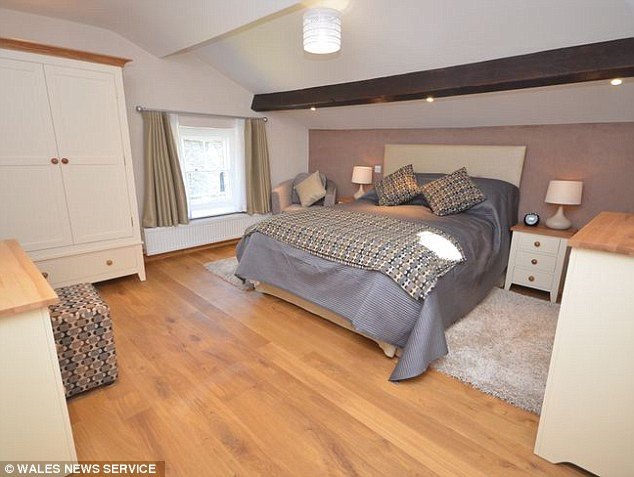
\includegraphics[width=0.70\textwidth]{type_c_conceptual_captions_02.png}
\caption{Conceptual Captions example 2 image sent to the model.}
\end{figure}

\promptbox{\textbf{Prompt for example 2.} Write one concise caption for the image; return only the caption text.}

\resultbox{\textbf{Reference for example 2.} the - bedroom stone cottage can sleep people\\\textbf{GPT-4o response.} Cozy bedroom with wooden flooring and modern decor. (incorrect)\\\textbf{GPT-4o score.} BLEU 0.1604}

\subsection*{FlyingThings3D Example}

\begin{figure}[H]
\centering
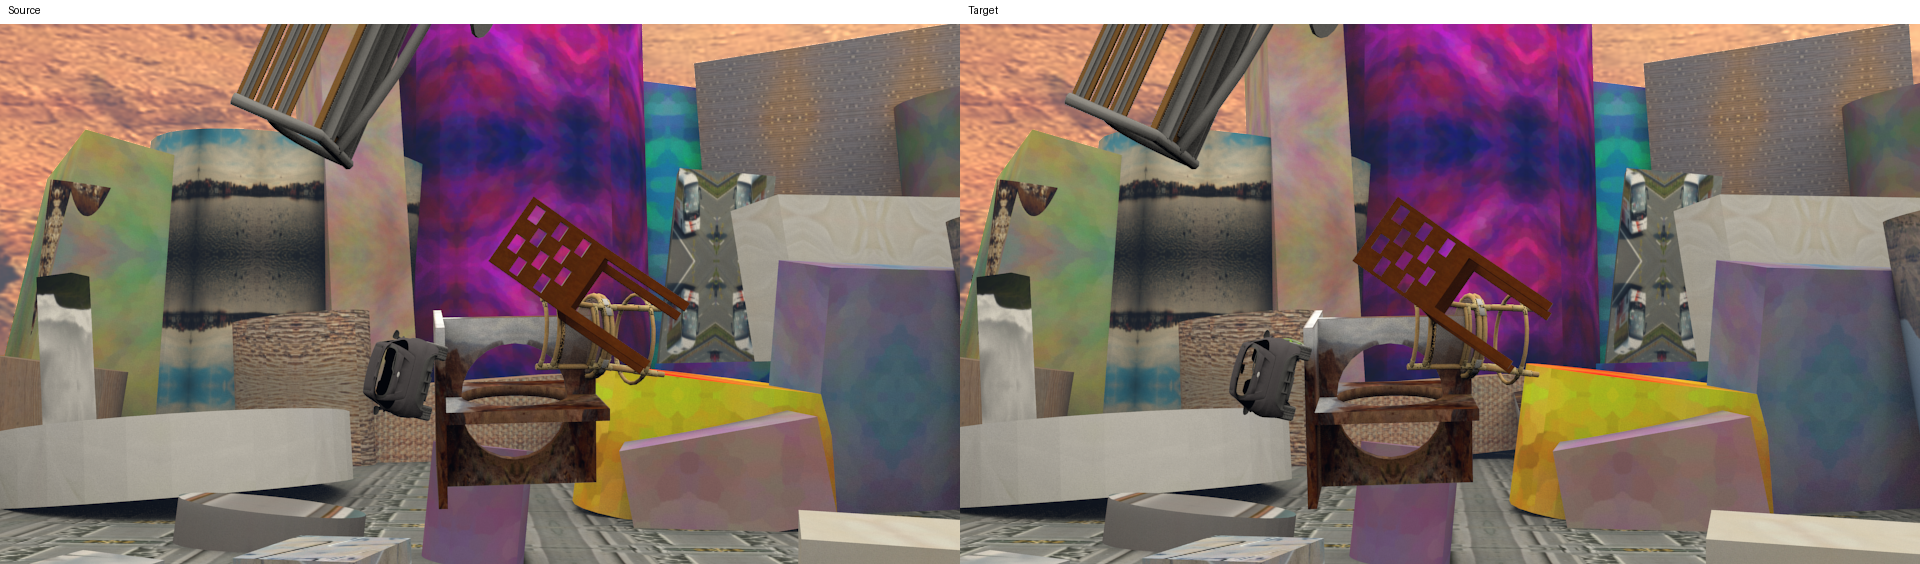
\includegraphics[width=0.70\textwidth]{type_a_flyingthings3d_03.png}
\caption{FlyingThings3D example 3 image sent to the model.}
\end{figure}

\promptbox{\textbf{Prompt for example 3.} Question: What part of the gray car is most visible?\\\textbf{Choices.}\\{} \textbf{A.} the front\\{} \textbf{B. the back}\\{} \textbf{C.} the side\\{} \textbf{D.} the top.}

\resultbox{\textbf{GPT-4o response.} C. the side (incorrect)}

\subsection*{MS COCO Example}

\begin{figure}[H]
\centering
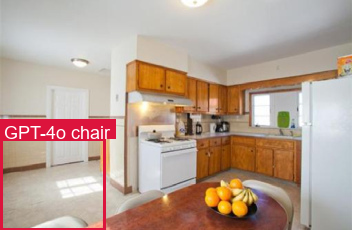
\includegraphics[width=0.70\textwidth]{type_b_mscoco_02_gpt4o_boxes.png}
\caption{MS COCO example 2 image sent to the model with GPT-4o predicted boxes drawn.}
\end{figure}

\promptbox{\textbf{Prompt for example 2.} Target class: chair. Detect every visible instance and return one normalized [x, y, width, height] box per line, or [] if none are visible.}

\resultbox{\textbf{Reference for example 2.} chair\\\textbf{GPT-4o response.} [0.0, 0.6, 0.3, 0.4] (incorrect)\\\textbf{GPT-4o boxes drawn in image.} chair: [0.00, 138.00, 105.60, 230.00]}

\subsection*{HQ-Edit Example}

\begin{figure}[H]
\centering
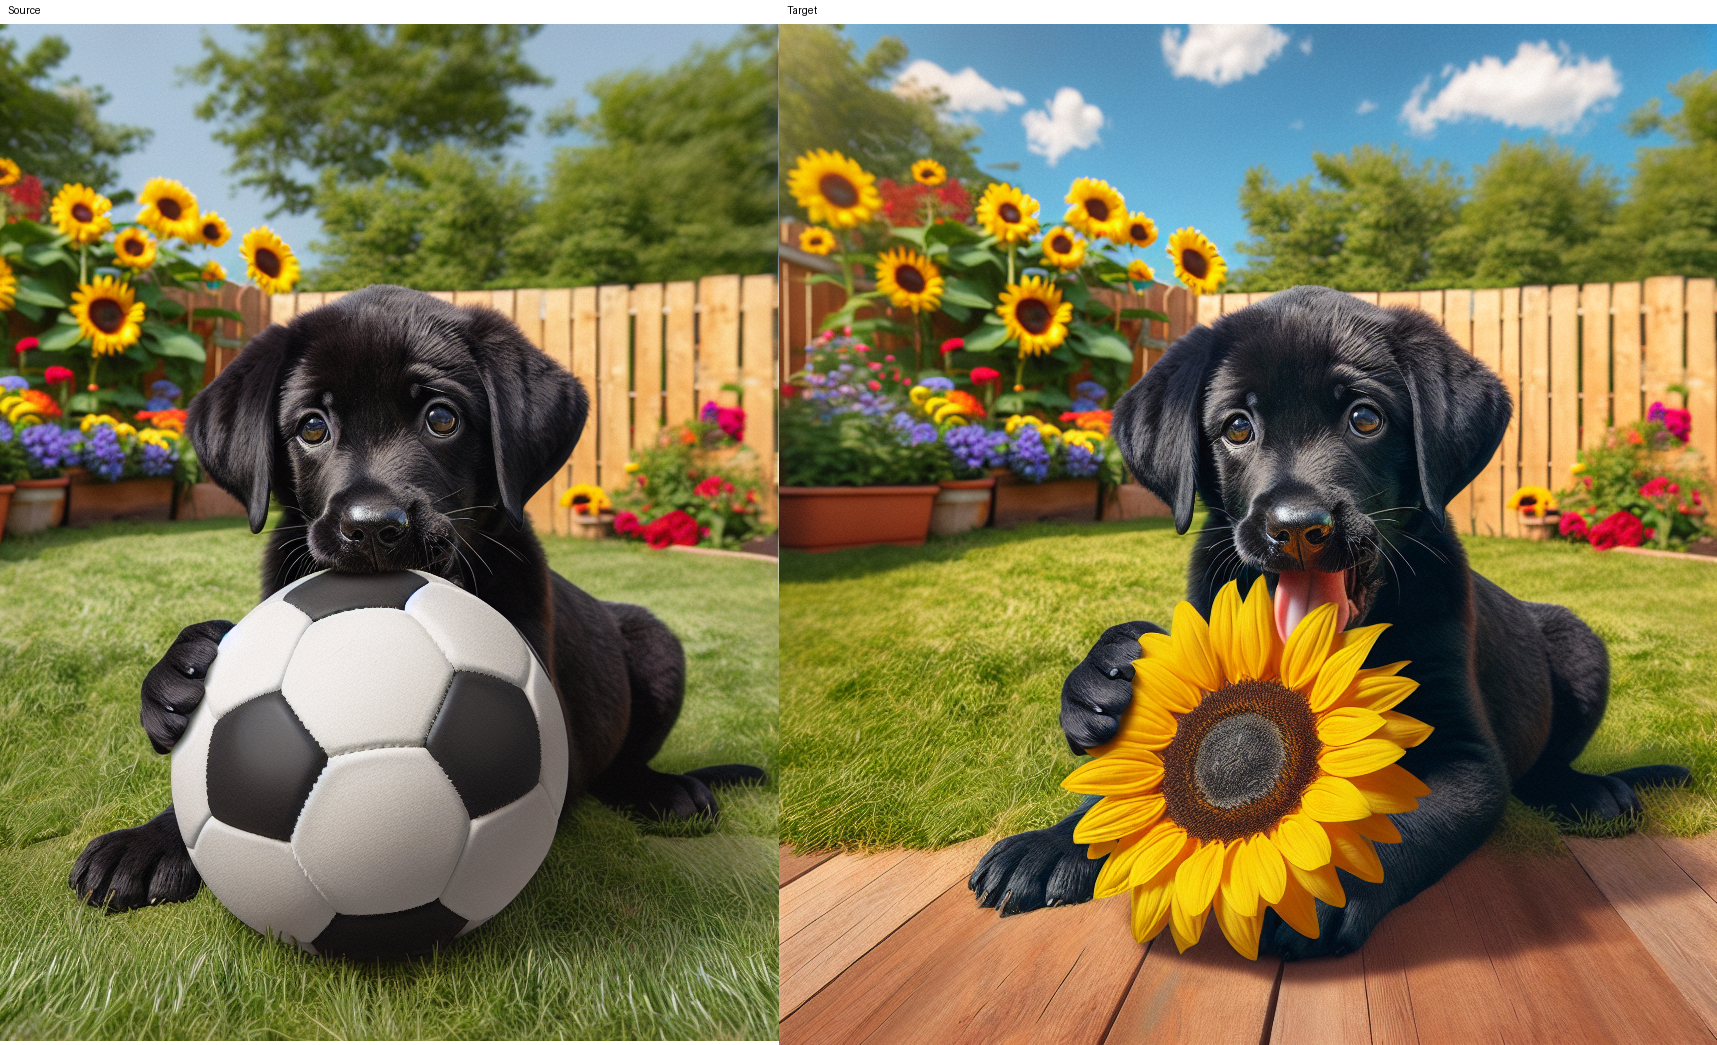
\includegraphics[width=0.70\textwidth]{type_e_hq_edit_05.png}
\caption{HQ-Edit example 5 image sent to the model.}
\end{figure}

\promptbox{\textbf{Prompt for example 5.} Identify which edit instruction produced Image B from Image A.\\\textbf{Choices.}\\{} \textbf{A.} Replace the soccer ball with a miniature sunflower that the puppy is holding in the same manner as the soccer ball.\\{} \textbf{B.} Replace the soccer ball with a miniature sunflower that the kitten is holding in the same manner as the soccer ball.\\{} \textbf{C. Replace the soccer ball with a giant sunflower that the puppy is holding in the same manner as the soccer ball.}\\{} \textbf{D.} Replace the soccer ball with a giant sunflower that the kitten is holding in the same manner as the soccer ball.}

\resultbox{\textbf{GPT-4o response.} C. Replace the soccer ball with a giant sunflower that the puppy is holding in (correct)}

\subsection*{DiffusionDB Example}

\begin{figure}[H]
\centering
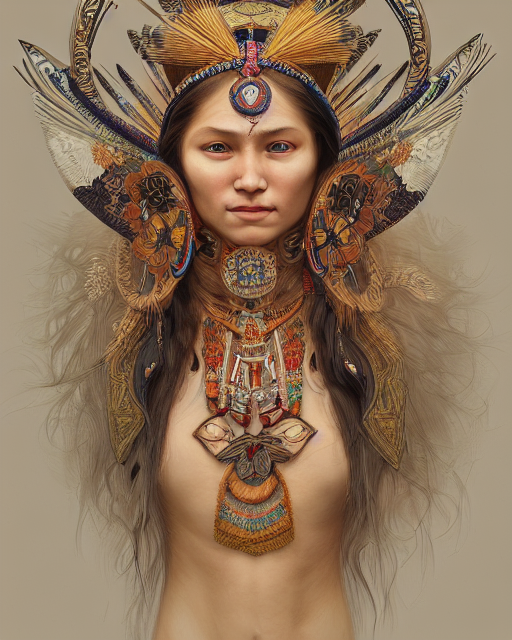
\includegraphics[width=0.70\textwidth]{type_g_diffusiondb_02.png}
\caption{DiffusionDB example 2 image sent to the model.}
\end{figure}

\promptbox{\textbf{Prompt for example 2.} Identify which prompt created the image.\\\textbf{Choices.}\\{} \textbf{A.} a renaissance portrait of dwayne johnson, art in the style of rembrandt!! intricate. ultra detailed, oil on canvas, wet - on - wet technique, pay attention to facial details, highly realistic, cinematic lightning, intricate textures, illusionistic detail,\\{} \textbf{B.} epic 3 d, become legend shiji! gpu mecha controlled by telepathic hackers, made of liquid, bubbles, crystals, and mangroves, houdini sidefx, perfect render, artstation trending, by jeremy mann, tsutomi nihei and ilya kuvshinov\\{} \textbf{C.} an airbrush painting of cyber war machine scene in area 5 1 by destiny womack, gregoire boonzaier, harrison fisher, richard dadd\\{} \textbf{D. portrait of a dancing eagle woman, beautiful blonde haired lakota sioux goddess, intricate, highly detailed art by james jean, ray tracing, digital painting, artstation, concept art, smooth, sharp focus, illustration, artgerm and greg rutkowski and alphonse mucha, vladimir kush, giger, 8 k.}}

\resultbox{\textbf{GPT-4o response.} D (correct)}

\subsection*{ImageNet Example}

\begin{figure}[H]
\centering
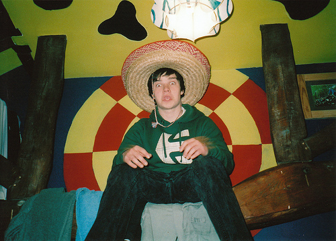
\includegraphics[width=0.70\textwidth]{type_l_imagenet1k_01.png}
\caption{ImageNet example 1 image sent to the model.}
\end{figure}

\promptbox{\textbf{Prompt for example 1.} Return exactly one label from the complete ImageNet-1K label list.}

\resultbox{\textbf{Reference for example 1.} sombrero\\\textbf{GPT-4o response.} sombrero (correct)}

\subsection*{TAD66K Rating Example}

\begin{figure}[H]
\centering
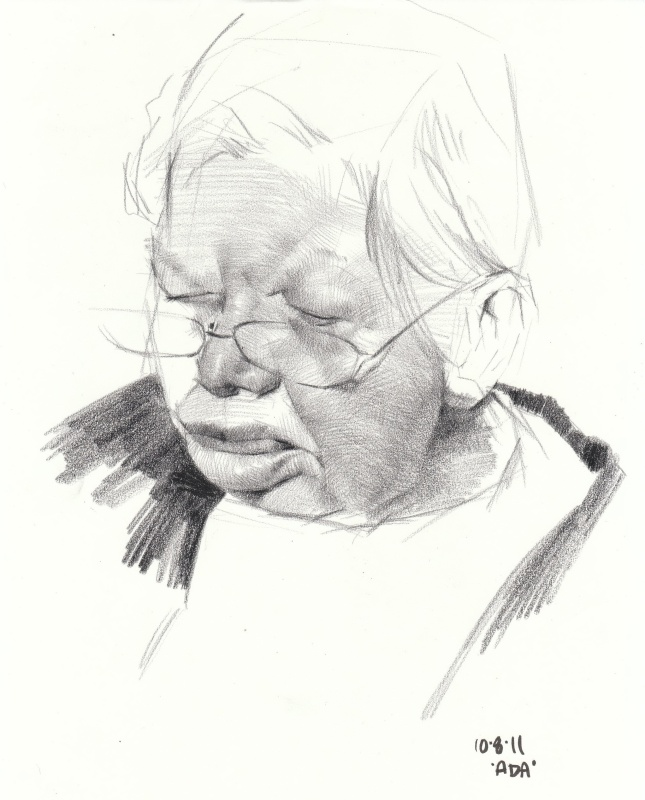
\includegraphics[width=0.70\textwidth]{type_r_tad66k_06.png}
\caption{TAD66K rating example 6 image sent to the model.}
\end{figure}

\promptbox{\textbf{Prompt for example 6.} Rate the overall aesthetic quality of this image from 1 to 10, where 1 is very poor and 10 is exceptional. Return exactly one integer from 1 to 10.}

\resultbox{\textbf{Reference for example 6.} 7\\\textbf{GPT-4o response.} 7 (correct)\\\textbf{GPT-4o absolute error.} 0}

\subsection*{Pick-a-Pic Preference Example}

\begin{figure}[H]
\centering
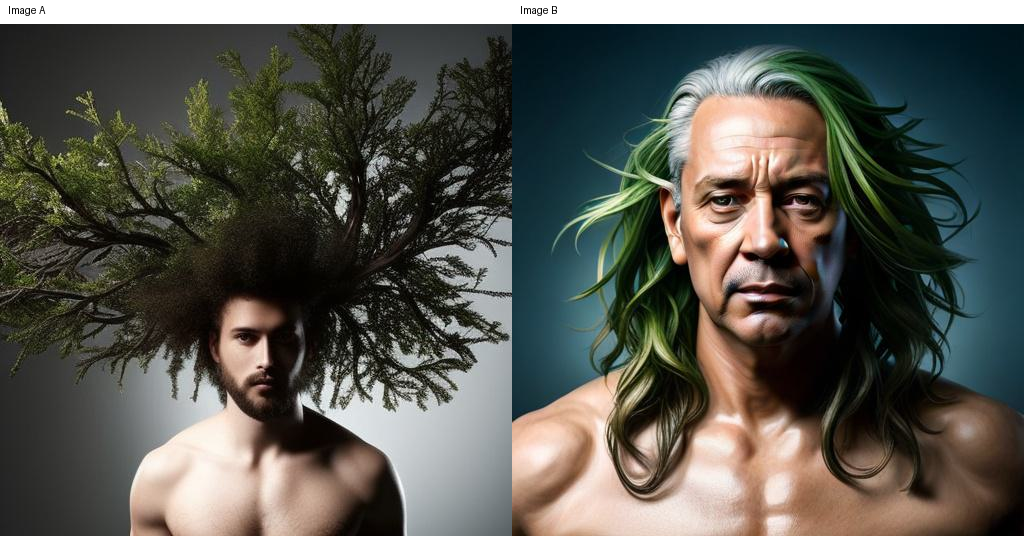
\includegraphics[width=0.70\textwidth]{type_p_pick_a_pic_04.png}
\caption{Pick-a-Pic preference example 4 image pair sent to the model.}
\end{figure}

\promptbox{\textbf{Prompt for example 4.} Which image is more aesthetically pleasing overall?\\\textbf{Choices.}\\{} \textbf{A.} Image A\\{} \textbf{B.} Image B\\{} Return only A or B.}

\resultbox{\textbf{Reference for example 4.} Image A\\\textbf{GPT-4o response.} A (correct)}


\begin{table}[H]
\centering
\small
\caption{The six benchmark types covered in this note.}
\begin{tabularx}{\textwidth}{@{}clXX@{}}
\toprule
\textbf{Type} & \textbf{Name} & \textbf{Example} & \textbf{Expected output} \\
\midrule
C & Captioning & Conceptual Captions & One concise free-form caption. \\
A & Answering Questions & FlyingThings3D & One answer to a visual question. \\
B & Bounding Box Detection & MS COCO & One normalized box per target object. \\
E & Editing Reconstruction & HQ-Edit & The edit instruction that explains a before--after pair. \\
G & Generating Reconstruction & DiffusionDB & The generation prompt that best explains the image. \\
L & Labeling & ImageNet & One class label from a fixed label set. \\
\bottomrule
\end{tabularx}
\end{table}

\section{Experimental setup and validity checks}

\section{Main results: GPT-4o vs Claude}

\section{Results by task family}

\section{Five-model comparison}

\section{Limitations}

\section{Conclusions and future work}

\end{document}
